\documentclass[10pt]{report}

\usepackage{amsmath}
\usepackage{amssymb}
\usepackage{graphicx}
\usepackage{helvet}

\setlength{\paperheight}{3in}
\setlength{\paperwidth}{4in}
\pdfpagewidth=\paperwidth
\pdfpageheight=\paperheight

\setlength{\textwidth}{3.5in}
\setlength{\textheight}{2.5in}

\setlength{\oddsidemargin}{-0.75in}
\setlength{\evensidemargin}{-0.75in}
\setlength{\topmargin}{-1.25in}

\newcommand{\sld}[1]{\newpage{\noindent\Large \underline{#1}}\vspace*{8pt}}
\newcommand{\itm}[1]{\vspace*{8pt}\noindent#1}
\newcommand{\itmb}{\itm{$\bullet$}\ }

\newcounter{gmlrx}
\newcounter{gmlry}
\newcommand{\gmnode}[3]{\put(#1,#2){\circle{20}}\put(#1,#2){\makebox(0,0){$#3$}}}
\newcommand{\gmplate}[5]{
\setcounter{gmlrx}{#1}\addtocounter{gmlrx}{#3}
\setcounter{gmlry}{#2}\addtocounter{gmlry}{-#4}
\put(#1,#2){\line(1,0){#3}}
\put(#1,#2){\line(0,-1){#4}}
\put(\value{gmlrx},\value{gmlry}){\line(-1,0){#3}}
\put(\value{gmlrx},\value{gmlry}){\line(0,1){#4}}
\setcounter{gmlrx}{#1}\addtocounter{gmlrx}{5}
\setcounter{gmlry}{#2}\addtocounter{gmlry}{-6}
\put(\value{gmlrx},\value{gmlry}){\makebox(0,0){$#5$}}
}



\begin{document}
\sf%
\vspace*{1pt}
\noindent
{\huge Ground Truth, \\[4pt]
Machine Learning, \\[4pt]
{\sf and the} \\[8pt]
Mechanical Turk}
\\[24pt]
{\Large Bob Carpenter}
(w.\ Emily Jamison, Breck Baldwin)
\\[4pt]
{\large\emph{Alias-i, Inc.}}



\sld{Supervised Machine Learning}

\begin{enumerate}
\item Define coding standard mapping inputs to outputs, e.g.:
\begin{itemize}
\footnotesize
\item English word $\rightarrow$ stem
\item newswire text $\rightarrow$ person name spans
\item biomedical text $\rightarrow$ genes mentioned
\end{itemize}
\item Collect inputs and code ``gold standard'' training data
\item Develop and train statistical model using data
\item Apply to unseen inputs
\end{enumerate}



\sld{Coding Bottleneck}

\begin{itemize}
\item Bottleneck is collecting training corpus
\item Commericial data's expensive (e.g.\ LDA, ELRA)
\item Academic corpora typically restrictively licensed
\item Limited to existing corpora
\item For new problems, use:
self, grad students, temps, interns, \ldots
\vspace*{12pt}
\item Mechanical Turk to the rescue
\end{itemize}

\newpage
\vspace*{36pt}
\noindent
{\huge Case Studies}

\sld{Case 1: Named Entities}

\hspace*{-24pt}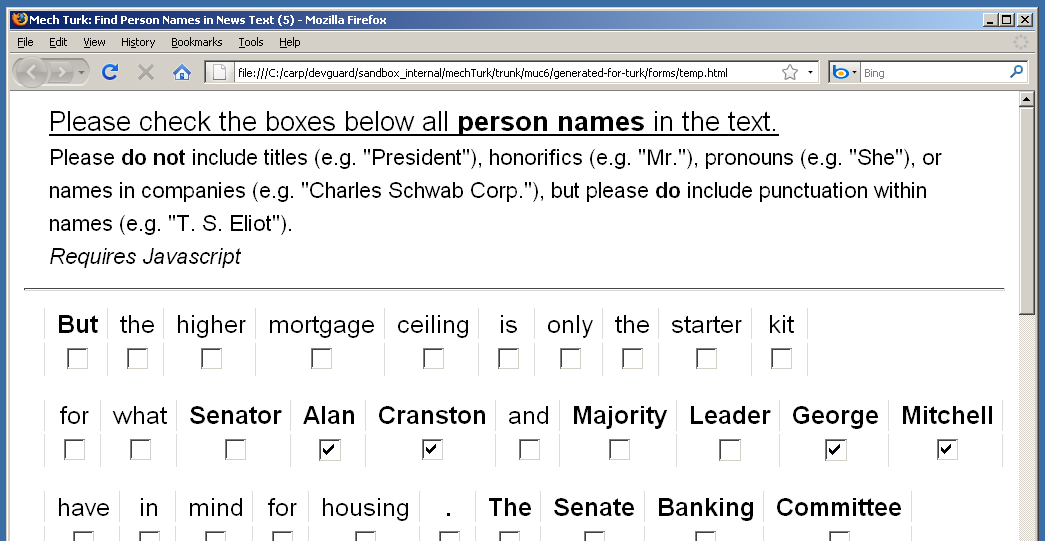
\includegraphics[width=1.05\textwidth]{pngs/big-ne-form.png}


\sld{Named Entities Worked}

\begin{itemize}
\item Conveying the coding standard
\begin{itemize}
\footnotesize
\item official MUC-6 standard dozens of pages
\item examples are key
\item (maybe a qualifying exam)
\end{itemize}

\item User Interface Problem
\begin{itemize}
\footnotesize
\item highlighting with mouse too fiddly (c.f. Fitt's Law)
\item one entity type at a time (vs. pulldown menus)
\item checkboxes (vs. highlighting spans)
\end{itemize}
\end{itemize}

\sld{Discussion: Named Entities}

\vspace*{-6pt}
\begin{itemize}
\item 190K tokens, 64K capitalized, 4K names
\item Less than a week at 2 cents/400 tokens
\item Turkers overall better than LDC data
\begin{itemize}
\footnotesize
\item Correctly Rejected:
{\tt\footnotesize Webster's, Seagram, Du Pont,
\\
Buick-Cadillac, Moon, erstwhile Phineas Foggs}
\item Incorrectly Accepted: {\tt\footnotesize Tass}
\item Missed Punctuation: {\tt\footnotesize J~E.~``Buster'' Brown}
\end{itemize}
\item Many Turkers no better than chance \\
(c.f.\ social psych by Yochai Benkler, Harvard)
\end{itemize}


\sld{Case 2: Morphological Stemming}

\hspace*{-24pt}
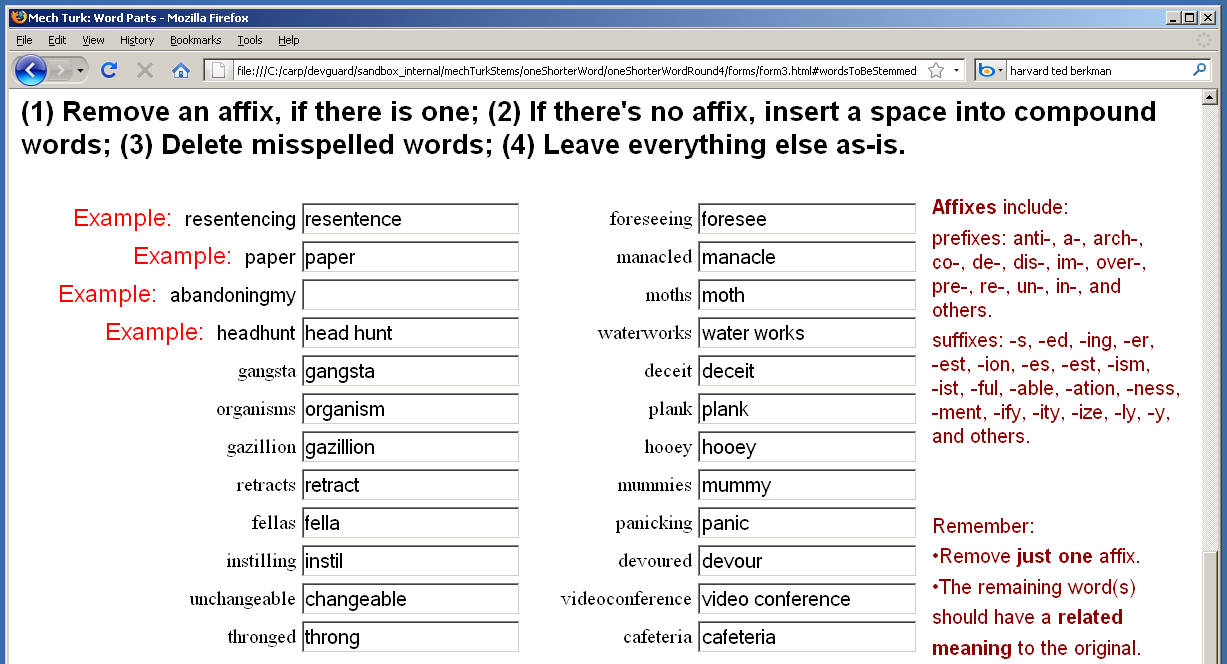
\includegraphics[width=1.05\textwidth]{pngs/stems-v4.png}


\sld{Morphological Stemming Worked}

\begin{itemize}
\vspace*{-8pt}
\item Three iterations on coding standard
\begin{itemize}
\footnotesize
\item simplified task to one stem
\end{itemize}

\item Four iterations on final standard instructions
\vspace*{-6pt}
\begin{itemize}
\footnotesize
\item added previously confusing examples
\end{itemize}

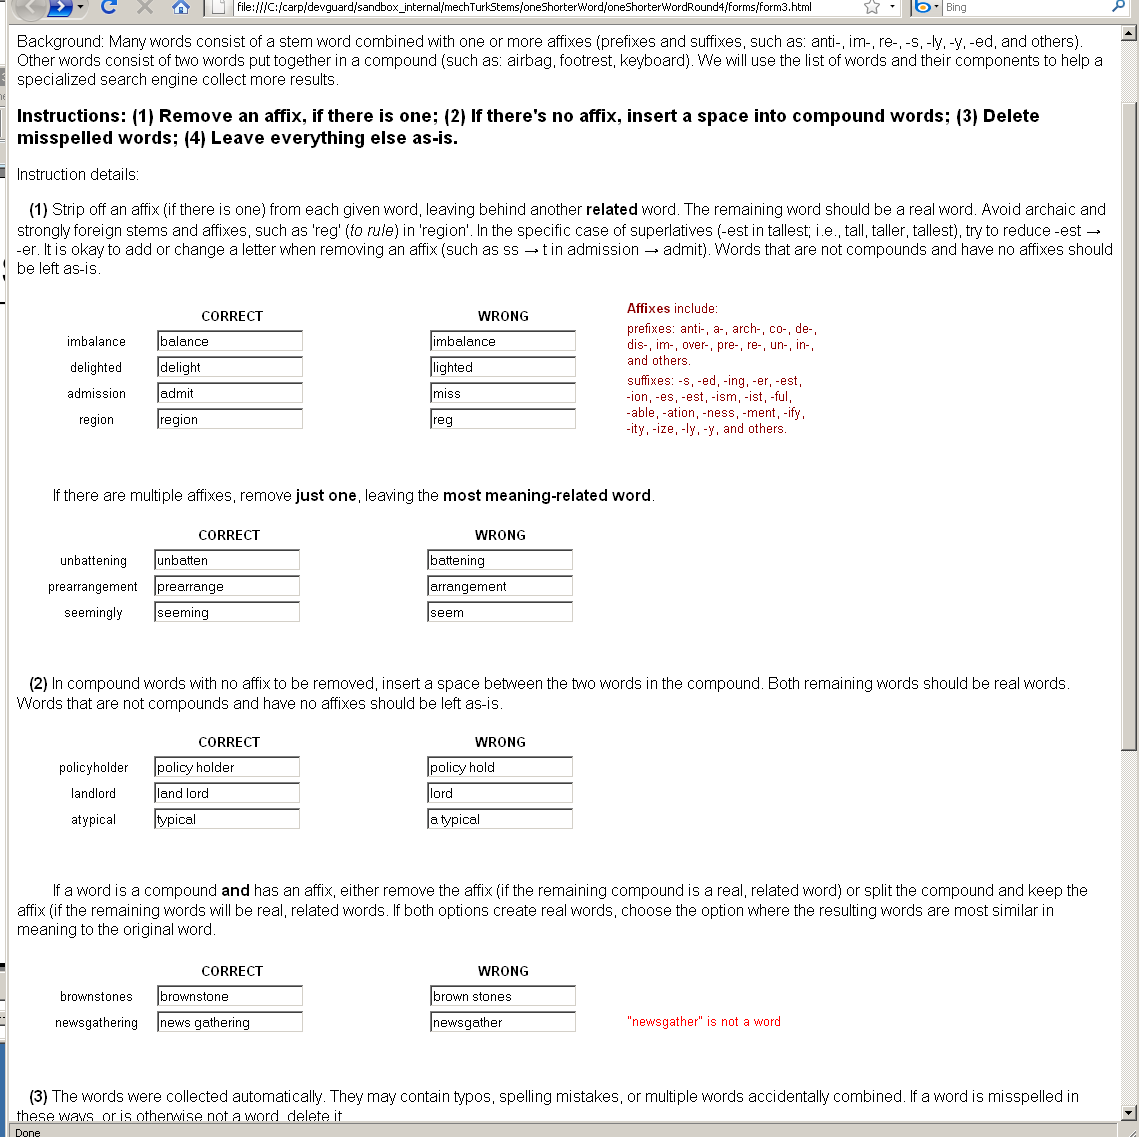
\includegraphics[width=0.2\textwidth]{pngs/stems-instrux.png}

\item Added qualifying test

\end{itemize}



\sld{Case 3: Gene Linkage}

\hspace*{-24pt}
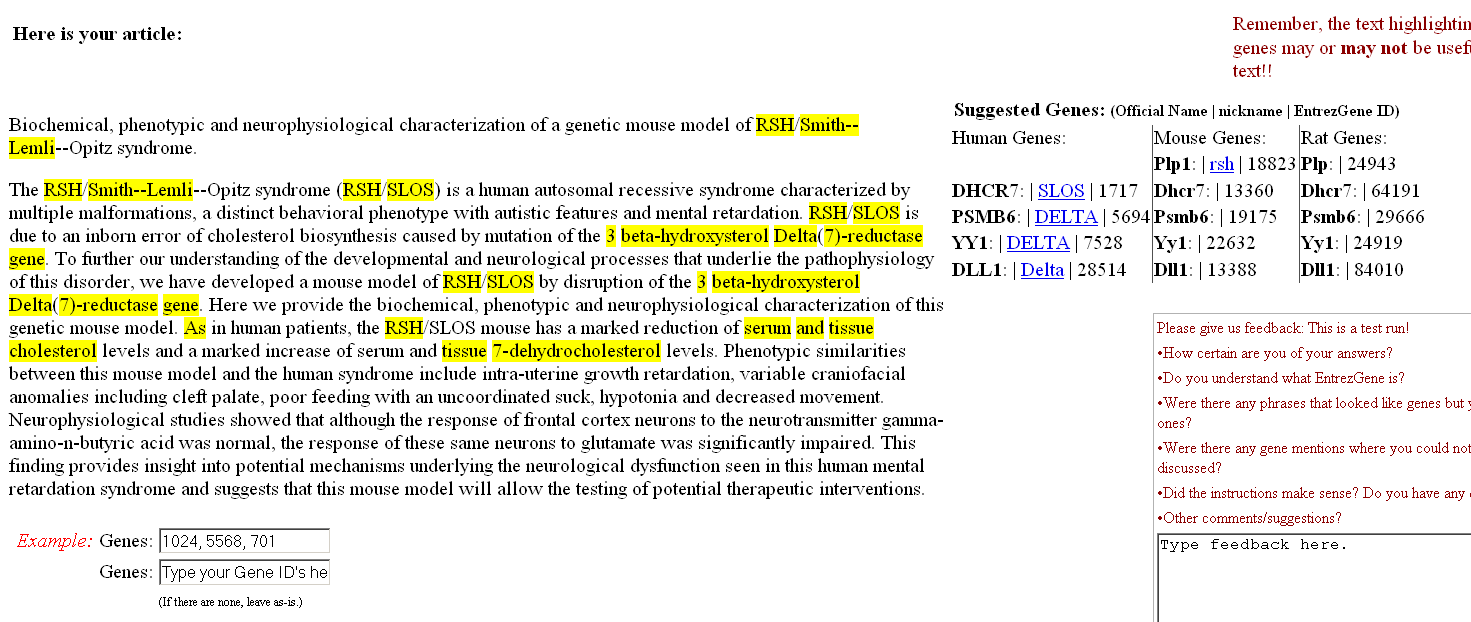
\includegraphics[width=1.05\textwidth]{pngs/gene-task.png}

\sld{Gene Linkage Failed}

\begin{itemize}
\item {\bfseries Could} get Turkers to pass qualifier
\item {\bfseries Could not} get Turkers to take task even at \$1/hit
\item Doing coding ourselves (5-10 minutes/HIT)
\vspace*{12pt}
\item How to get Turkers do these complex tasks?
\begin{itemize}
\footnotesize
\item Low concentration tasks done quickly
\item Compatible with studies of why Turkers Turk
\end{itemize}
\end{itemize}



\newpage
\vspace*{36pt}
\noindent
{\huge Inferring Gold Standards}


\sld{Voted Gold Standard}

\begin{itemize}
\item Turkers vote
\item Label with majority category
\item Censor if no majority
\end{itemize}


\sld{Some Labeled Data}

\begin{itemize}
\item Seed the data with cases with known labels
\item Use known cases to estimate coder accuracy
\item Vote with adjustment for accuracy
\item Requires relatively large amount of items for
\begin{itemize}
\footnotesize
\item estimating accuracies well
\item liveness for new items
\end{itemize}
\item Gold may not be as pure as requesters think
\item Some preference tasks have no ``right'' answer
\begin{itemize}
\footnotesize
\item e.g. Bing vs. Google, Facestat, Colors, ...
\end{itemize}
\end{itemize}


\sld{Estimate Everything}

\begin{itemize}
\item Gold standard labels
\item Coder accuracies
    \begin{itemize}
\footnotesize
      \item sensitivity (false negative rate; misses)
      \item specificity (false positive rate; false alarms)
      \item imbalance indicates bias; high values accuracy
    \end{itemize}
\item Coding standard difficulty
    \begin{itemize}
\footnotesize
        \item average accuracies
        \item variation among coders
    \end{itemize}
\item Item difficulty (important, but not enough data)
\end{itemize}


\sld{Benefits of Estimation}

\begin{itemize}
\item Full Bayesian posterior inference
\begin{itemize}
\footnotesize
\item probabilistic ``gold standard''
\item compatible with Bayesian machine learning
\end{itemize}
\item Works better than voting with threshold
\begin{itemize}
\footnotesize
\item largest benefit with few Turkers/item
\item evaluated with known ``gold standard''
\end{itemize}
\item Compatible with adding gold standard cases
\end{itemize}


\sld{Why we Need Task Difficulty}

\begin{itemize}
\item What's your estimate for:
\begin{itemize}
\footnotesize
\item a baseball player who goes 12 for 20?
\item a market that goes down 9 out of 10 days?
\item a coin that lands heads 3 out of 10 times?
\item \ldots
\end{itemize}
\item Smooth estimates for coders with few items
\item Hierarchical model of accuracy prior
\end{itemize}


\sld{Soft Gold Standard}

\begin{itemize}
\item Is 24 karat gold standard even possible?
\item Some items are really marginal
\item Traditional approach
\begin{itemize}
\footnotesize
\item censoring disagreements
\item adjudicating disagreements (revise standard)
\item adjudication may not converge
\end{itemize}
\vspace*{12pt}
\item Posterior uncertainty can be modeled
\end{itemize}



\sld{Active Learning}

\begin{itemize}
\item Choose most useful items to code next
\item Balance two criteria
\begin{itemize}
\footnotesize
\item high uncertainty
\item high typicality (how to measure?)
\end{itemize}
\item Can get away with fewer coders/item
\item May introduce sampling bias
\end{itemize}


\sld{Code-a-Little, Learn-a-Little}

\begin{itemize}
\item Semi-automated coding
\item System suggests labels
\item Coders correct labels
\item Much faster coding
\item But may introduce bias
\end{itemize}



\newpage
\vspace*{36pt}
\noindent
{\huge Statistical Inference Model}


\sld{5 Dentists Diagnosing Cavities}

{\footnotesize
\begin{tabular}{cr|cr|cr}
{\it Dentists} & {\it Count} &
{\it Dentists} & {\it Count} &
{\it Dentists} & {\it Count}
\\ \hline
00000 & 1880 & 10000 & 22 & 00001 & 789 \\
10001 & 26 & 00010 & 43 & 10010 & 6 \\
00011 & 75 & 10011 & 14 & 00100 & 23 \\
10100 & 1 & 00101 & 63 & 10101 & 20 \\
00110 & 8 & 10110 & 2 & 00111 & 22 \\
10111 & 17 & 01000 & 188 & 11000 & 2 \\
01001 & 191 & 11001 & 20 & 01010 & 17 \\
11010 & 6 & 01011 & 67 & 11011 & 27 \\
01100 & 15 & 11100 & 3 & 01101 & 85 \\
11101 & 72 & 01110 & 8 & 11110 & 1 \\
01111 & 56 & 11111 & 100
\end{tabular}
}


\sld{Posteriors for Dentist Accuracies}

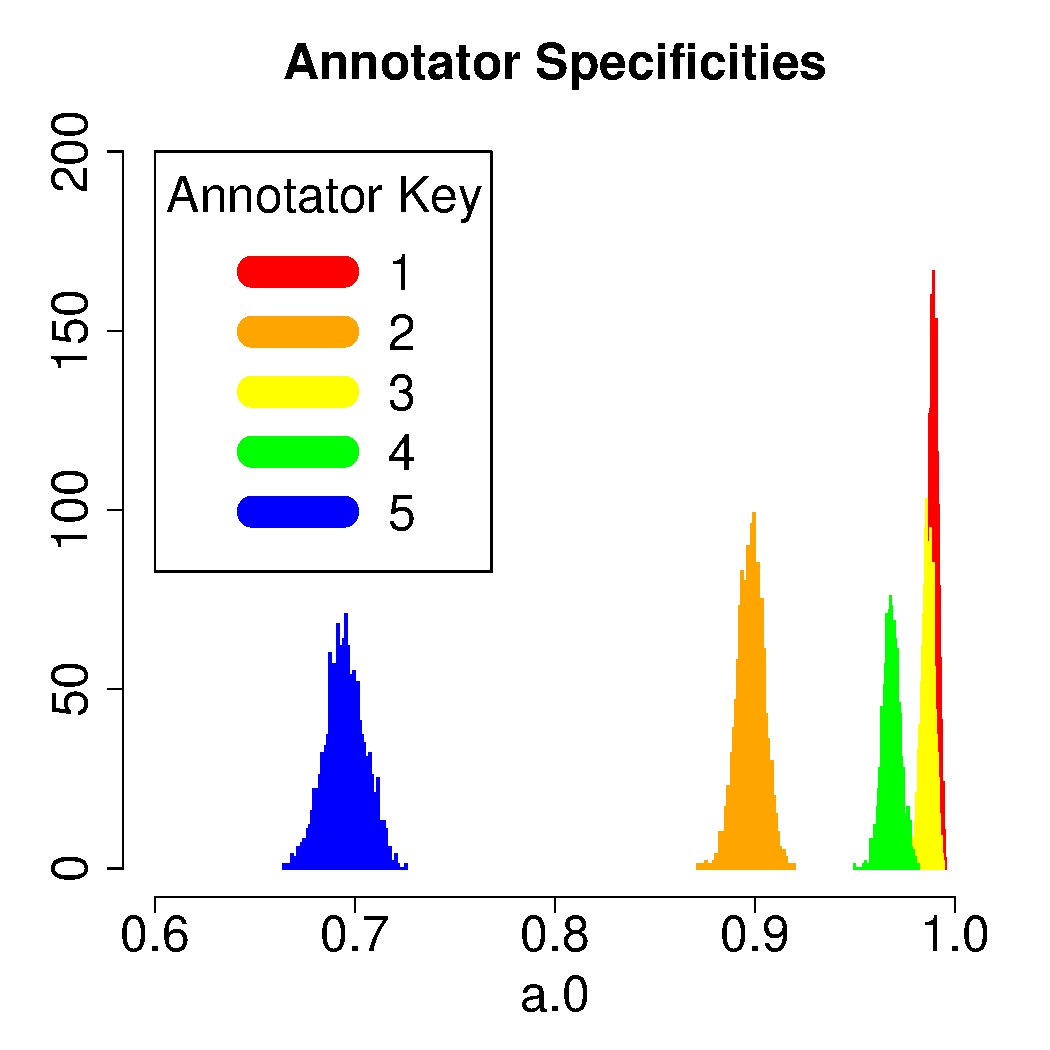
\includegraphics[width=0.4\textwidth]{pngs/a-0-hist.pdf}
\ \ \
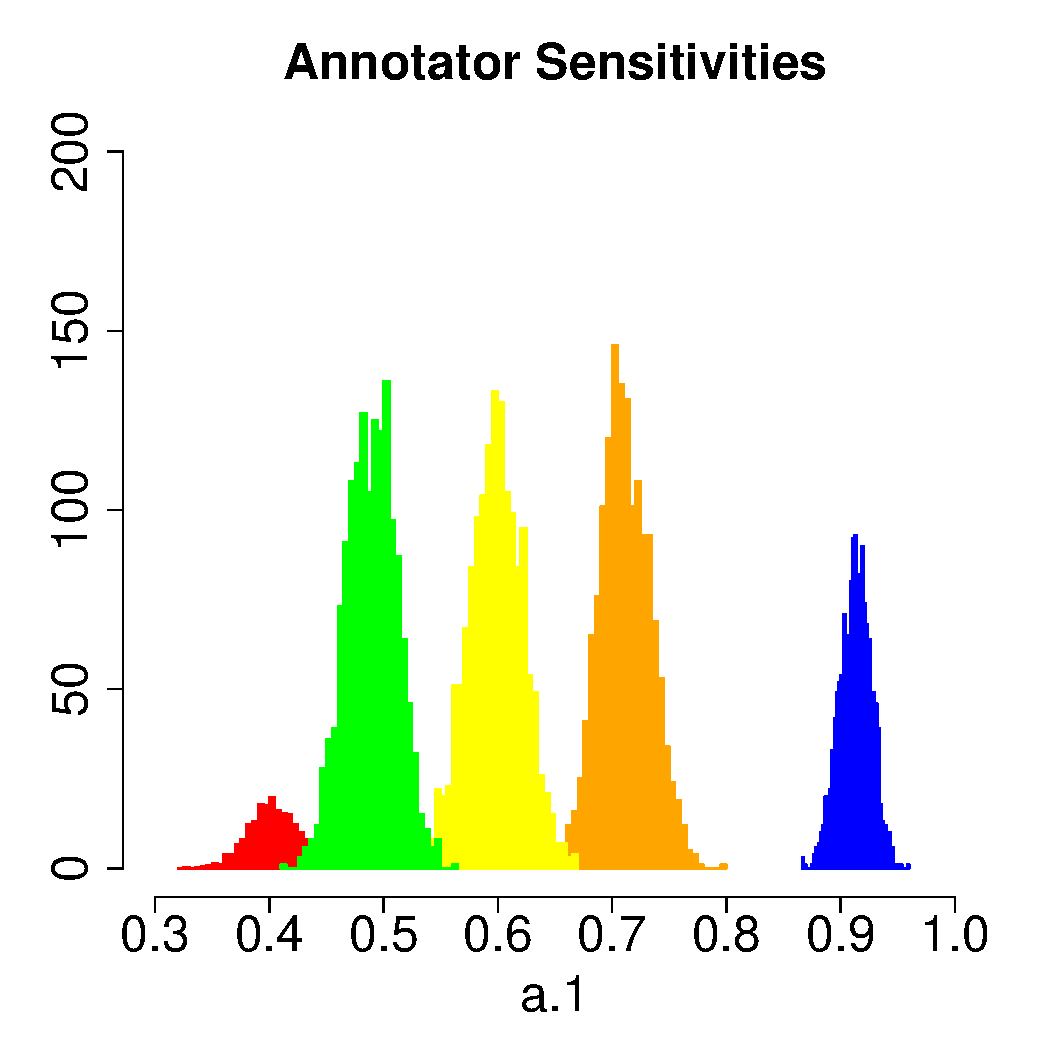
\includegraphics[width=0.4\textwidth]{pngs/a-1-hist.pdf}

\begin{itemize}
\item Posterior density vs. point estimates (e.g. mean)
\end{itemize}


\sld{Posteriors for Dentistry Data Items}

\hspace*{-24pt}
\begin{tabular}{ll}
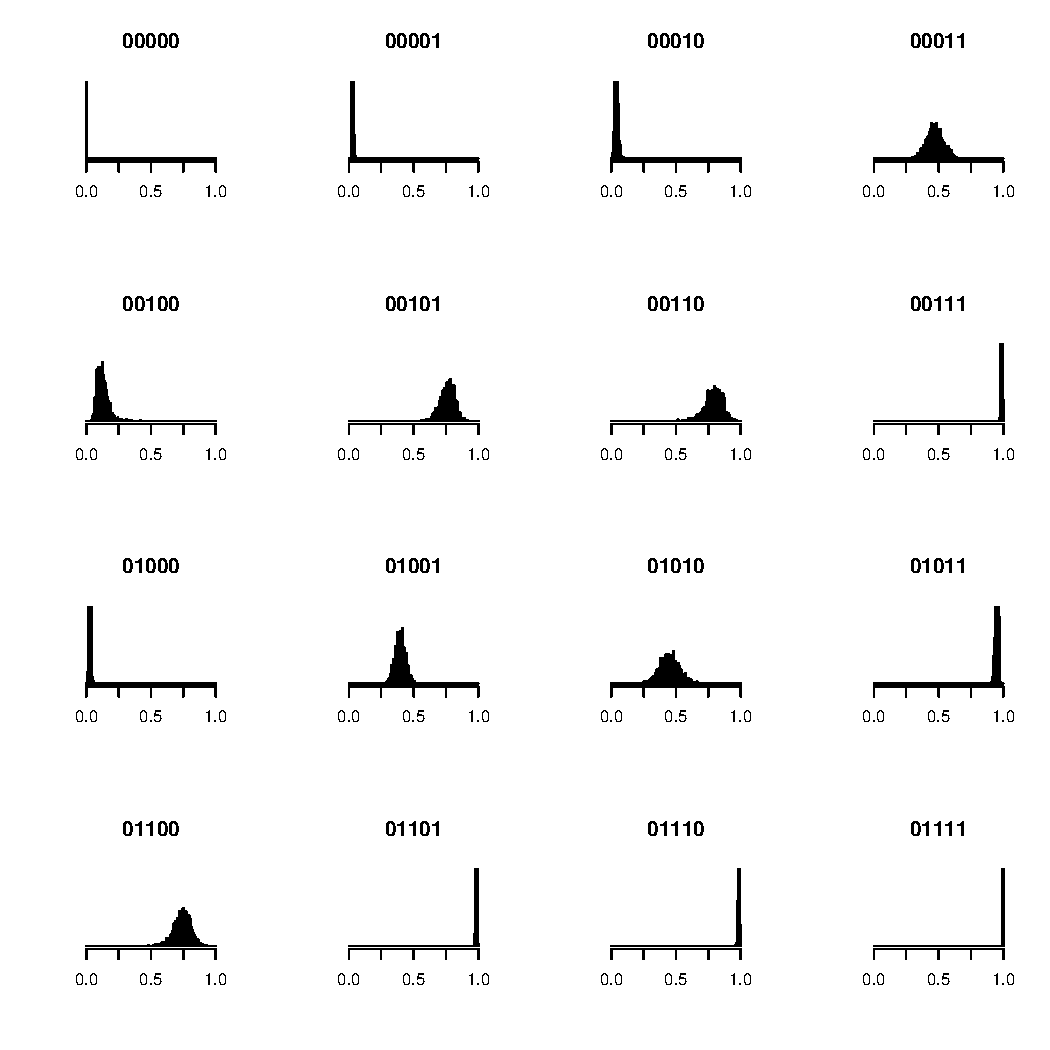
\includegraphics[width=0.5\textwidth]{pngs/model-4-cat-posteriors-dentistry.pdf}
&
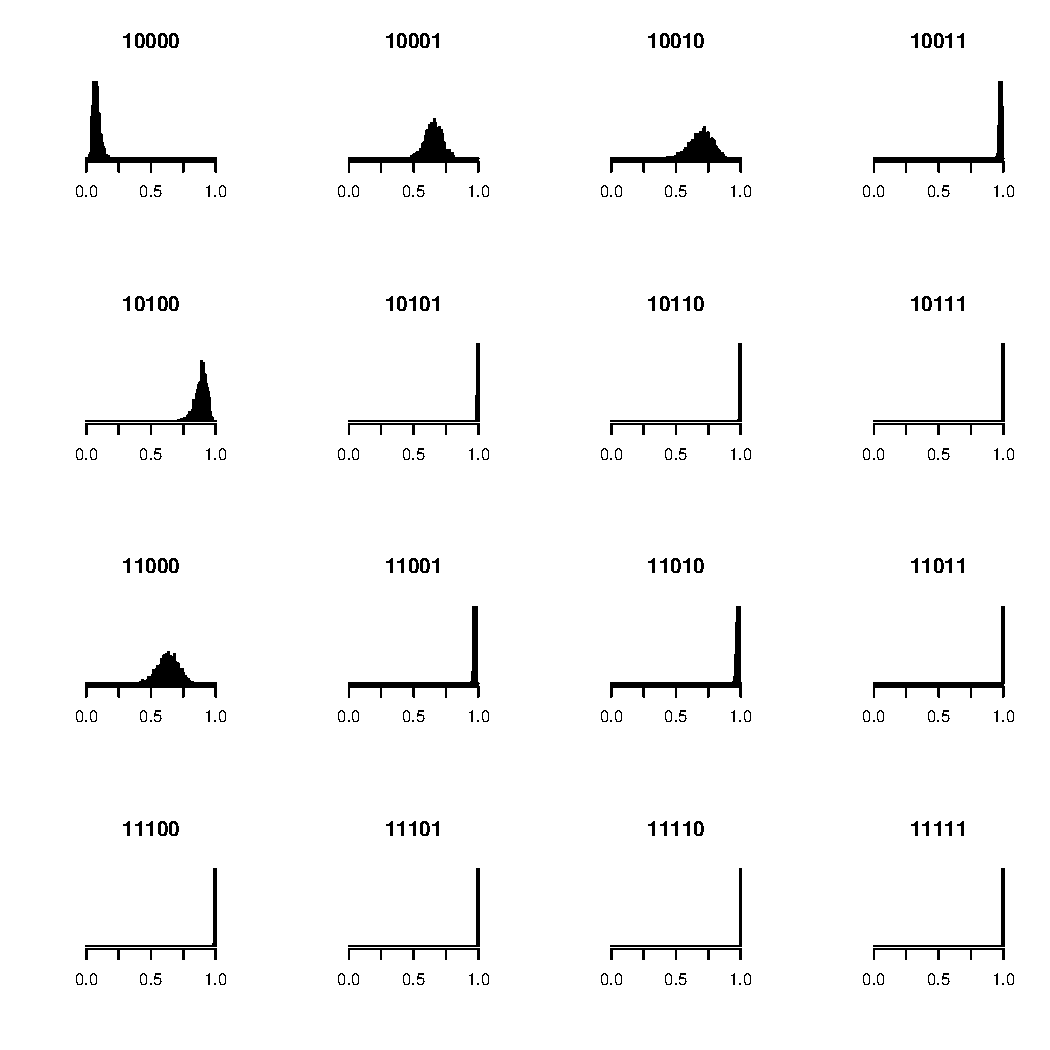
\includegraphics[width=0.5\textwidth]{pngs/model-4-cat-posteriors-dentistry-2.pdf}
\end{tabular}

Accounts for bias, so very different from simple vote!





\sld{Beta-Binomial ``Random Effects''}


\begin{picture}(195,145)

\gmnode{57.5}{132.5}{\alpha_0}
\gmnode{97.5}{132.5}{\beta_0}
\gmnode{142.5}{132.5}{\alpha_1}
\gmnode{182.5}{132.5}{\beta_1}
\gmnode{77.5}{92.5}{\theta_{0,j}}
\gmnode{162.5}{92.5}{\theta_{1,j}}
\gmnode{10}{30}{\pi}
\gmnode{55}{30}{c_i}
\gmnode{120}{30}{x_k}

\put(57.5,122.5){\vector(1,-1){19.75}}  % alpha_0 to theta_0_j
\put(97.5,122.5){\vector(-1,-1){19.75}} % beta_0 to theta_0_j
\put(142.5,122.5){\vector(1,-1){19.75}}  % alpha_1 to theta_1_j
\put(182.5,122.5){\vector(-1,-1){19.75}} % beta_1 to theta_1_j
\put(20,30){\vector(1,0){25}}  % \pi to c_i
\put(65,30){\vector(1,0){45}}  % c_i to x_k
\put(77.5,82.5){\vector(1,-1){42.5}}  % theta_0_j to x_k
\put(162.5,82.5){\vector(-1,-1){42.5}}  % theta_1_j to x_k

\gmplate{30}{55}{50}{50}{I}
\gmplate{95}{55}{50}{50}{K}
\gmplate{45}{115}{150}{45}{J}

\end{picture}

\sld{Sampling Notation}

Coders don't all code the same items

\vspace*{-8pt}
{\footnotesize
\begin{eqnarray*}
c_i & \sim & \mathsf{Bernoulli}(\pi)
\\
a_{0,j} & \sim & \mathsf{Beta}(\alpha_0,\beta_0)
\\
a_{1,j} & \sim & \mathsf{Beta}(\alpha_1,\beta_1)
\\
x_k & \sim & \mathsf{Bernoulli}(c_{i_k} a_{1,j_k}
                                        + (1 - c_{i_k}) (1 - a_{0,j_k}))
\\[8pt]
\pi & \sim & \mathsf{Beta}(1,1)
\\
\alpha_0/(\alpha_0 + \beta_0) & \sim & \mathsf{Beta}(1,1)
\\
\alpha_0 + \beta_0 & \sim & \mathsf{Polynomial}(-5/2)
\\
\alpha_1/(\alpha_1 + \beta_1) & \sim & \mathsf{Beta}(1,1)
\\
\alpha_1 + \beta_1 & \sim & \mathsf{Polynomial}(-5/2)
\\
\end{eqnarray*}}


\sld{Posterior for Coding Difficulty/Variance}

These are posteriors from a simulation with cross-hairs giving ``true''
answer:

\hspace*{-24pt}
\begin{tabular}{ll}
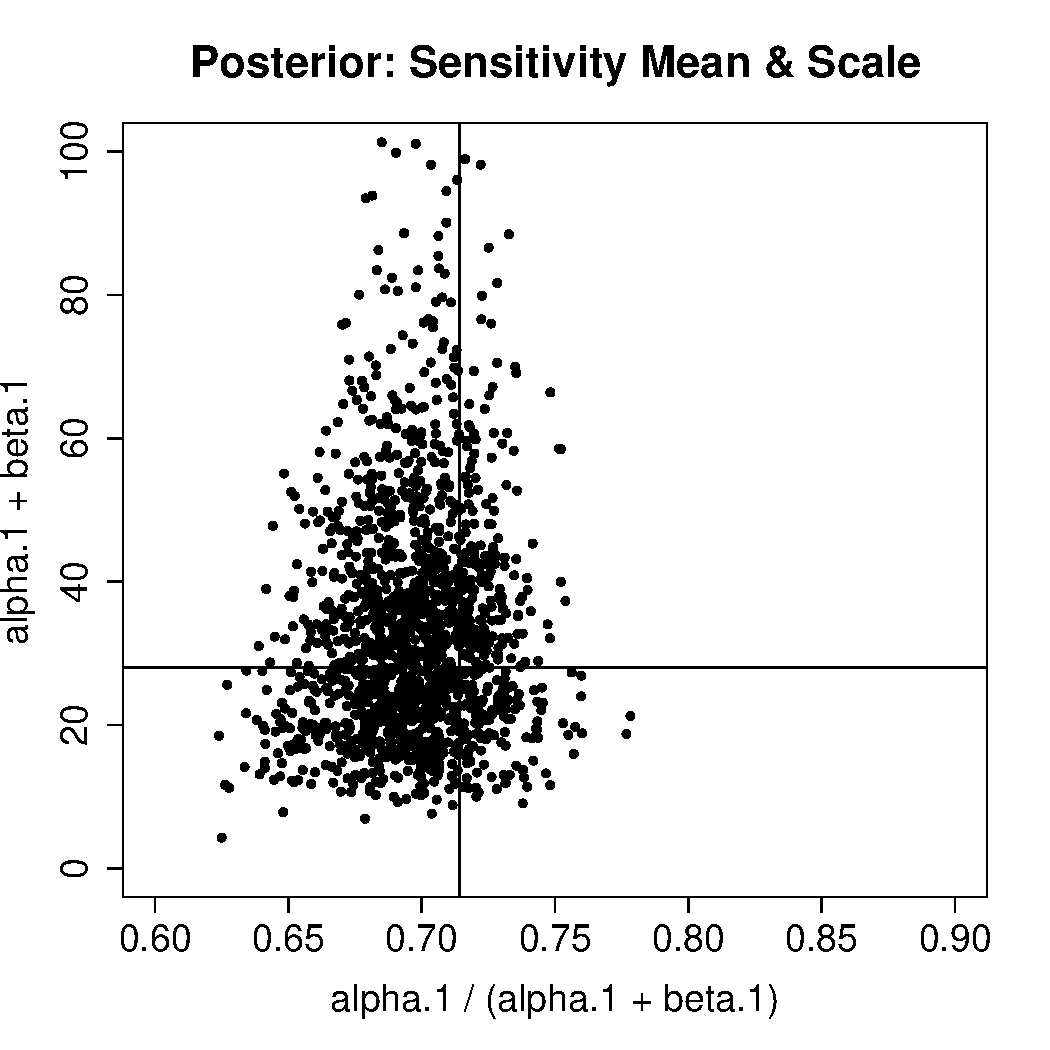
\includegraphics[width=0.5\textwidth]{pdf/beta-binomial-anno-scatter-sens.pdf}
&
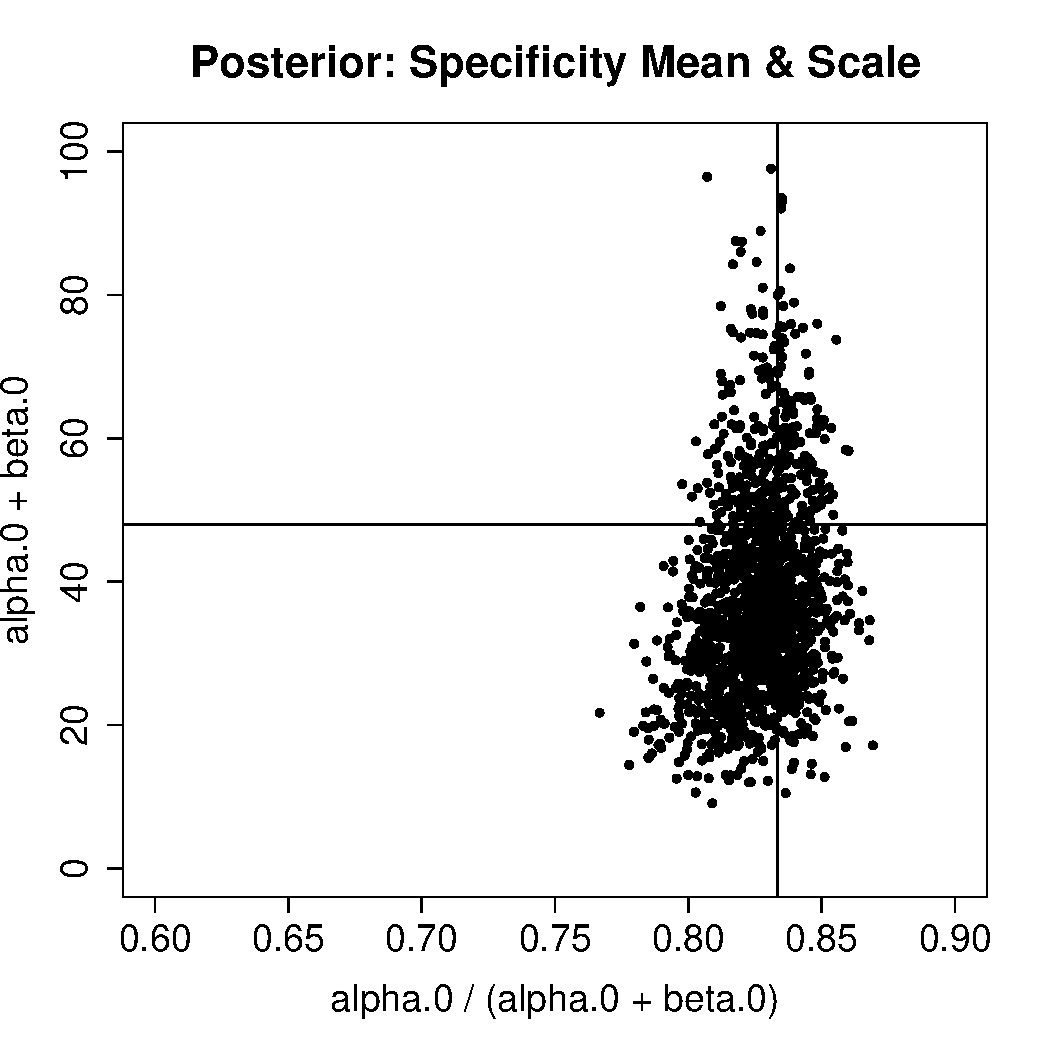
\includegraphics[width=0.5\textwidth]{pdf/beta-binomial-anno-scatter-spec.pdf}
\end{tabular}


\sld{Extending Model}

\begin{itemize}
\item Task difficulty
\begin{itemize}
\footnotesize
\item Logistic Item-Response models
\item Need more than 5-10 coders/item for tight posterior
\end{itemize}
\item Easy to extend coding types
\begin{itemize}
\footnotesize
\item Multinomial responses
\item Ordinal responses (e.g. Likert 1-5 scale)
\item Scalar responses
\end{itemize}
\end{itemize}

\sld{The End}

\begin{itemize}
\item References
\begin{itemize}
\item {\tt http://lingpipe-blog.com}
\end{itemize}
\item Contact
\begin{itemize}
\item
{\tt carp@alias-i.com}
\end{itemize}
\item
R/BUGS Code Subversion Repository
\begin{itemize}
\item {\tt http://alias-i.com/lingpipe/sandbox}
\end{itemize}
\end{itemize}

\end{document}

